\section{Light Shift}

Next we will start with showing off. A little bitt at least. We will put three lights in a row and lighten one of them up each time we press the button.

It would be much easier to do this with 8 lights, but here we are. We will keep the existing circuit as untouched as possible and, not at last, we are constantly on he search for a challenge.

So here is the enhanced circuit:

\begin{figure}[htbp]
  \centering
  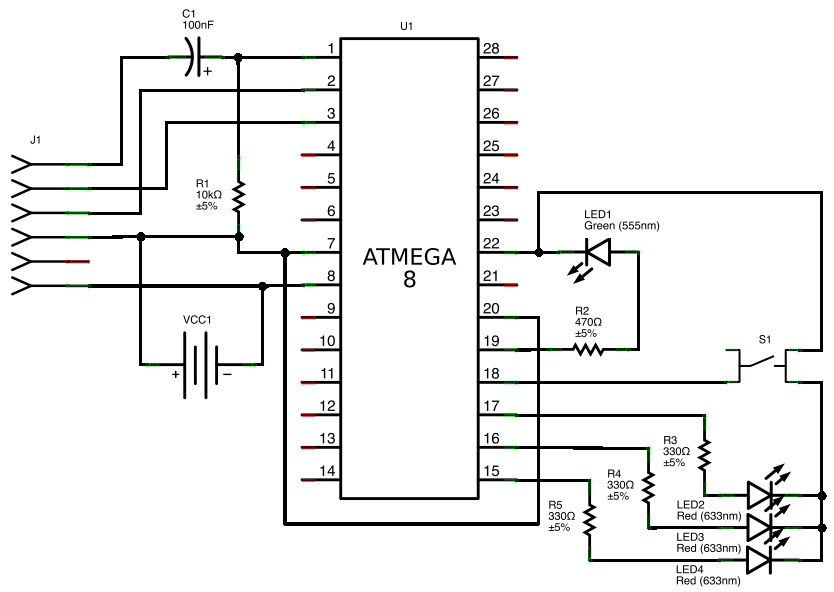
\includegraphics[width=120mm]{LED/S010_light-shift_Circuit_schema.png}
  \caption{Light Shift Schema}
  \label{atmega8-light-shift-schema}
\end{figure}


And here is the code:

\begin{lstlisting}
; LED/S010_light-shift.asm

.DEVICE atmega8


.equ ctlIO         = DDRB
.equ prtIO         = PORTB
.equ pinIO         = PINB

.equ bitSignal     = 5
.equ bitInput      = 4
.equ bitLightStart = 3

.equ mskLightShift = 0x0E

.equ LOW           = 0
.equ HIGH          = 1

.def bStatus       = r16
.def bTemp         = r17
.def bData         = r18


.org 0x0000
            rjmp    start


start:
            ldi     bTemp,        mskLightShift | 1 << bitSignal
            out     ctlIO,        bTemp
            ldi     bTemp,        1 << bitInput | 1 << bitSignal
            out     prtIO,        bTemp

            ldi     bStatus,      HIGH

main:
            sbic    pinIO,        bitInput
            rjmp    led_keep
            tst     bStatus
            breq    led_ok
            clr     bStatus

            in      bData,        pinIO
            mov     bTemp,        bData
            andi    bData,        0xFF - mskLightShift
            ori     bData,        1 << bitInput

            andi    bTemp,        mskLightShift
            lsr     bTemp
            andi    bTemp,        mskLightShift
            brne    shift_ok
            ldi     bTemp,        1 << bitLightStart
shift_ok:
            or      bData,        bTemp
            out     prtIO,        bData

            rjmp    led_ok
led_keep:
            ldi     bStatus,      HIGH
led_ok:
            rjmp    main
\end{lstlisting}

As you can see, we have some changes to the former code. This is, in the hole, because we will deal with four instead of one lights. One light (the one we toggled last time) will serve as signal light, lighting up after out micro controller has finished booting. The other will used to shift the light. In our case, this means, we start off with one light ON and each time we press our button the next light lights up whilst the former active light shuts off.

Our code reflects this at the first look with more constants and more named registers. Already we are using 10\% of all registers present and 20\% of all registers usable for generic purpose. This is bad news! Hopefully our resource consumption will not grow with constant speed.

Names for values (not resources) we need besides the ones from the former sample are

\begin{lstlisting}
.equ bitLightStart = 3     ; as in  0b00001000

.equ mskLightShift = 0x0E  ; builds 0b00001110
\end{lstlisting}

\texttt{bitLightStart} is the number of the pin on the output port where the first LED of our LED chain resides. The other LEDs are expected to use the two lower pins (2 and 1). Pin B0 on the \at can be found on the other side of the chips, so for our physical breadboard circuit it's a bit too complicated to use it.

Please remember, such decisions are no fun. In reality you may sometimes be driven to compensate in software for simplification of hardware as PCB layout, different chips and so on. So we accept this situation as example of what may happen in real life.

\texttt{mskLightShift} is a bit mask containing bits ate all pins of the output port where our light chain is connected to. We need such a bit mask because we need to shift the 'LED ON' bit around but won't shift any other bits found in the port data.

Named registers (resources) we need in addition are:
 
\begin{lstlisting}
.def bTemp         = r17
.def bData         = r18
\end{lstlisting}

\texttt{bTemp} will be used to shift our 'lED ON' bit around but \texttt{bData} has to give us the 'big picture' about our ports status. First before, second after shifting the 'LED ON' bit.

We start, as usual, by initialising the micro controller where it needs to be initialised. This time, we need to set all pins on our port the same time because the alternative is (for the moment) not acceptable. So we build a bit mask to send it to our IO ports data direction register (DDR):

\texttt{mskLightShift} combined with \texttt{1 << bitSignal} makes \texttt{0b00101110}. Sending this byte to DDRx will set pins 1, 2, 3, 5 to output and all other pins to input mode.

\begin{lstlisting}
start:
            ldi     bTemp,        mskLightShift | 1 << bitSignal
            out     ctlIO,        bTemp
            ldi     bTemp,        1 << bitInput | 1 << bitSignal
            out     prtIO,        bTemp
\end{lstlisting}

Then we need to do three things by sending a byte to PORTx:

\begin{itemize}
  \item Switch ON LED on pin 5 (\texttt{bitSignal})
  \item Set pin 4, our input pin, to 'pulled up' (\texttt{bitInput})
  \item Set all other pins to off/offline
\end{itemize}

All this is done by mixing all active bits together and sending the mix \texttt{(0b00110000)} to the port. After doing so the signal LED is on, the light chain is off. Until \texttt{clr bStatus} nothings more has changed. Also the rest with and after label \texttt{led\_keep} is kept the same.

The changed part is this:

\begin{lstlisting}
            in      bData,        pinIO
            mov     bTemp,        bData
            andi    bData,        0xFF - mskLightShift
            ori     bData,        1 << bitInput

            andi    bTemp,        mskLightShift
            lsr     bTemp
            andi    bTemp,        mskLightShift
            brne    shift_ok
            ldi     bTemp,        1 << bitLightStart
shift_ok:
            or      bData,        bTemp
            out     prtIO,        bData
\end{lstlisting}

All magic resides in these lines. It's not too much, so we simply explain it sequentially.

We need to get the ports state and unfortunately we have to understand more about this than is good for the program. We have to send back the whole data byte, modified only in the part where the LED chain state changed. BUT (!) we also need to ensure, our input pin keeps his pull up resistor active. Otherwise we loos our connection to the outer world!

Next we need to split the read byte/data in two parts. The one containing constant data and the other one containing the bits to be shifted.

Phase one therefore copies \texttt{bData} to \texttt{bTemp}, then masks out all bits dealer with in the bit shifting process and finally adding/regenerating the 'pull up' bit for port \texttt{bitInput}.

Phase two masks out all bits not related to the bis shifting operation, shifts the remaining bit and masks the result again with the same mask. If this operation leads to a result of ZERO/EQ/NULL, then we have shifted out our bit and need to insert a new bit at the start position inside the byte \texttt{bitLightStart}.

Phase three then combines our static bits with our manipulated one and put all together to our combined input/output port.
